\begin{figure}[h]
    \centering
    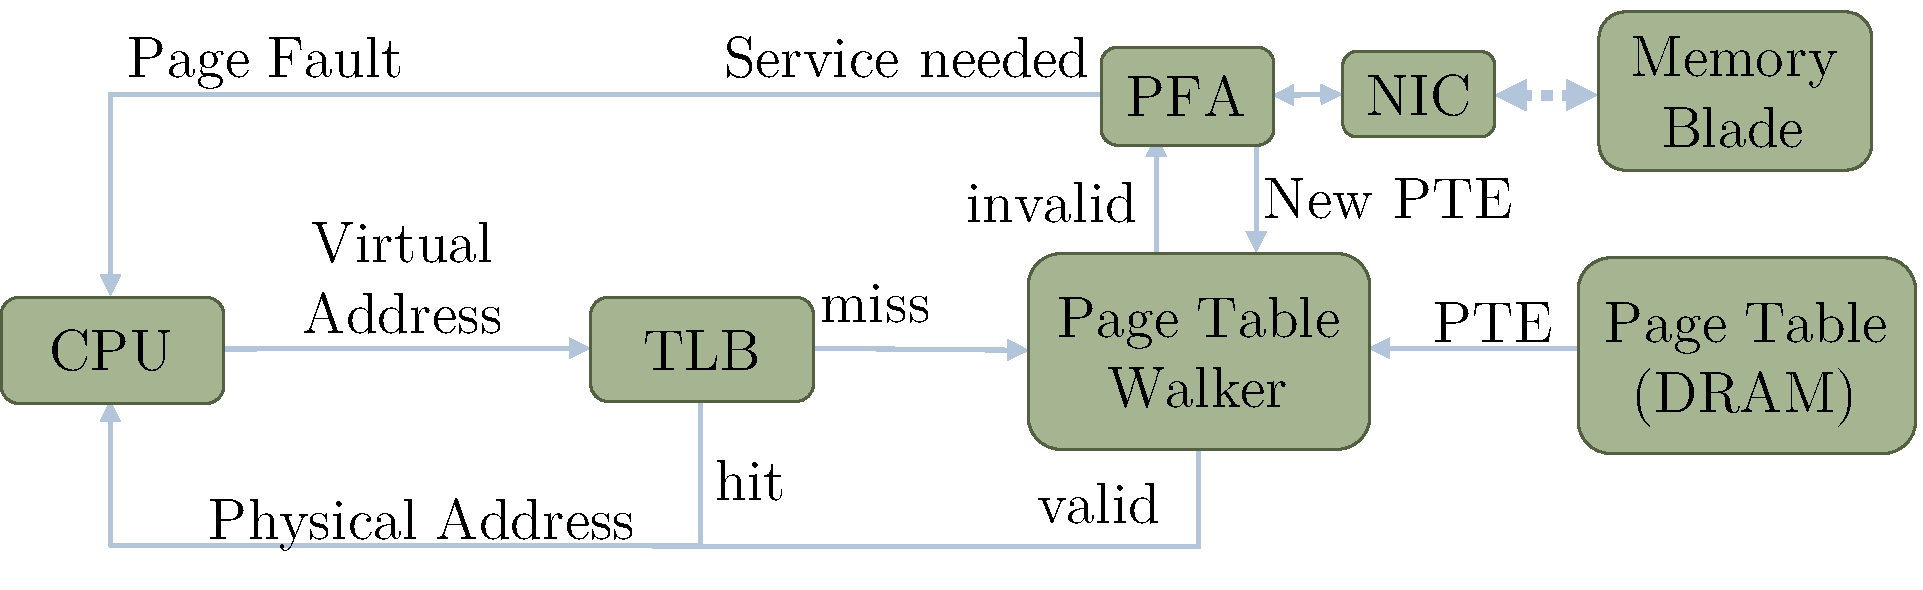
\includegraphics[width=0.9\columnwidth]{figs/generic_pfa.pdf}
    \vspace{-5mm}
    \caption{Paging with the PFA. Instead of an invalid PTE causing a trap to the OS (as in figure \ref{fig:generic_paging}), invalid pages are passed to the PFA to be fetched from remote memory. The PFA may still cause a trap if it cannot handle the request (e.g., full queues).}
    \label{fig:pfa_generic}
\end{figure}

Much of the work done during a page fault, while important, does not strictly
need to occur in order for the application thread to make progress. For
example, allocating free frames or updating page meta-data could be performed at
any time. Other tasks may be more efficient in hardware than in the OS; the
walking of page-tables for example. We propose a hardware accelerator that
performs only the bare-minimum of copying a remote page into a pre-allocated
frame, updating the relevant PTE, and restarting the application (figure
\ref{fig:pfa_generic}).

While this does not eliminate the need for software management of page meta-data
(here referred to as \gls{bookkeeping}), it does provide considerable flexibility
to the OS in how such \glspl{task} get scheduled. Figure
\ref{fig:bookkeeping_timeline} illustrates the difference from the perspective
of the OS. One immediate benefit is that the OS can schedule this bookkeeping
thread on idle resources, e.g. while the application is blocked on I/O.
Another benefit is that bookkeeping tasks can now be batched. Batching improves
cache locality and amortizes context switch overheads. 

\begin{figure}[h]
    \centering
    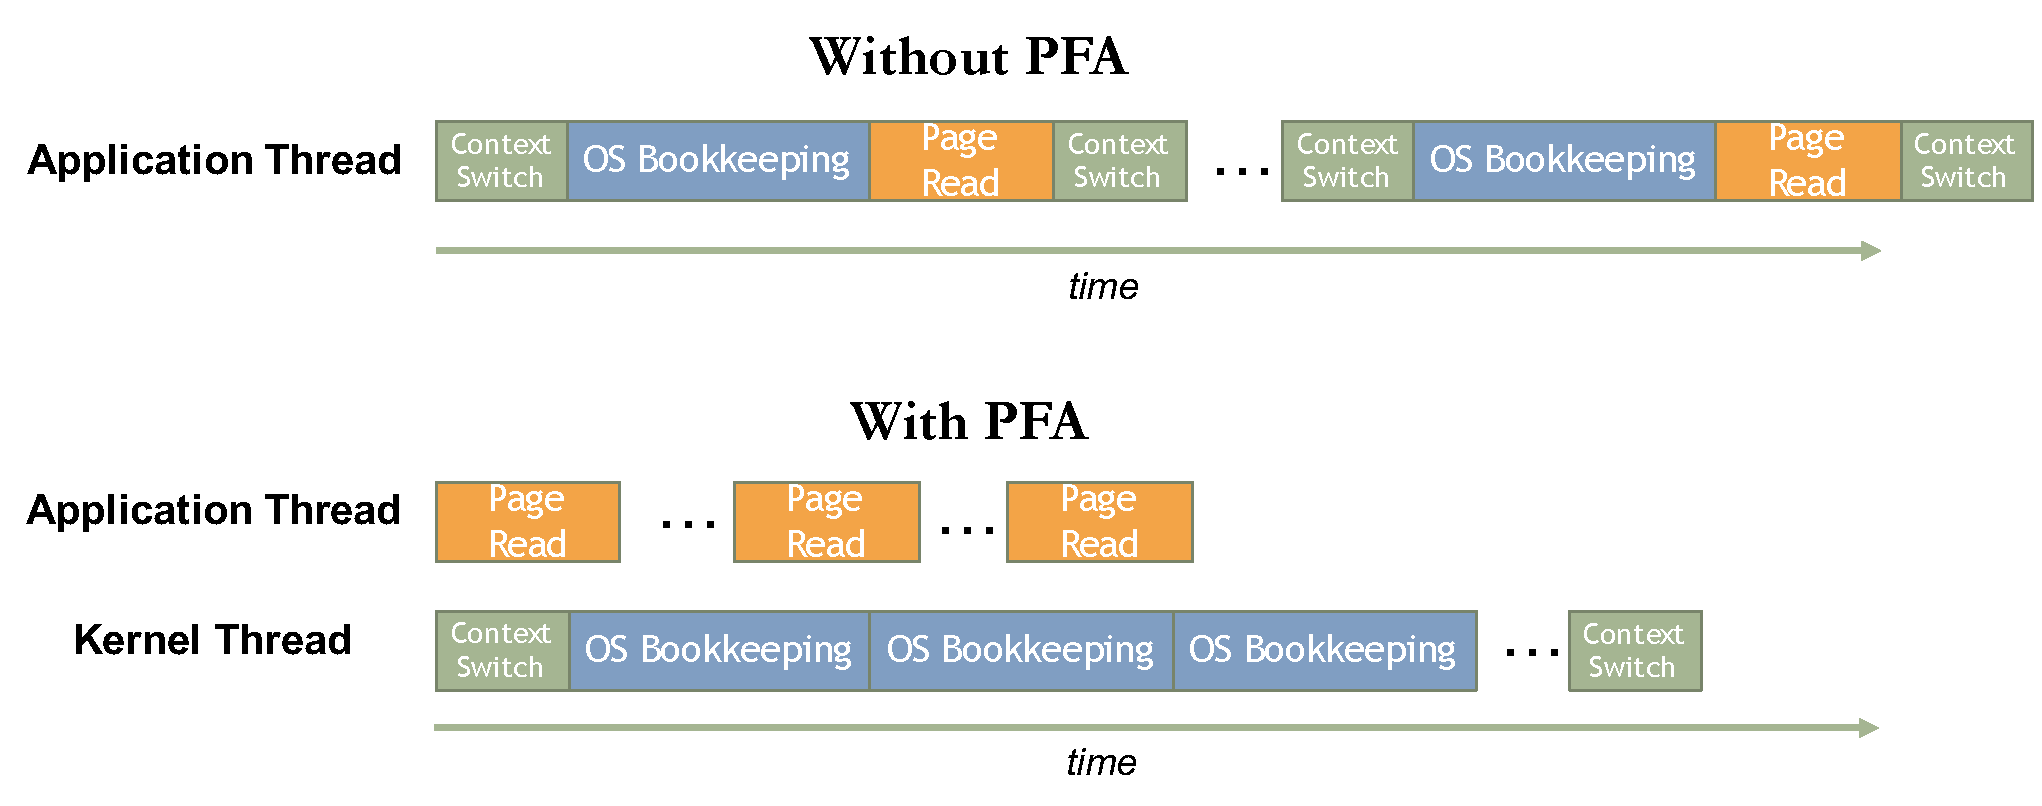
\includegraphics[width=\columnwidth]{figs/bookkeeping_timeline.pdf}
    \vspace{-5mm}
    \caption{Timeline of page-fault processing with and without the PFA. Without the PFA, the OS must be invoked on every page miss and perform various data structure look ups to decide how to handle the fault. The PFA allows this bookkeeping to occur any time after the fetch in a separate kernel thread. Only the actual page read must occur before the application can be restarted.}
    \label{fig:bookkeeping_timeline}
\end{figure}

\FloatBarrier
